\documentclass[a4paper,12pt]{article}
\usepackage[hmargin=2cm,top=4cm,headheight=65pt,footskip=45pt]{geometry}
\usepackage[utf8]{inputenc}
\usepackage{graphicx}
\usepackage[hidelinks]{hyperref}
\usepackage{array}
\usepackage{lastpage}
\usepackage{lipsum}
\usepackage{fancyvrb}
\usepackage{color}
\usepackage{fancyhdr}
\usepackage{amsmath}
\usepackage{enumitem}
\usepackage{titlesec}
\usepackage{floatrow}
\newfloatcommand{capbtabbox}{table}[][\FBwidth]

\definecolor{customGray}{RGB}{128,128,128}
%\definecolor{Eblue}{RGB}{0,21,87}
%\definecolor{Eblue}{rgb}{0.2, 0.2, 0.6}
\definecolor{Eblue}{rgb}{0.0, 0.18, 0.39}
%==============Header & Footnote==============

\pagestyle{fancy}
\renewcommand{\headrulewidth}{0pt}
\fancyhead[C,CO,L,LO,R,RO]{}
\fancyhead[C]{%
          \begin{tabular}{|m{3.0cm}|m{10.0cm}|m{2.5cm}|}
          \hline
          \centering\vspace{1.75mm}
\includegraphics[scale=0.275]{logo.pdf} &
          \centering
          {\footnotesize {\sf UNIVERSIDAD EAFIT\\ SCHOOL OF ENGINEERING\\
          \vspace{-1mm}DEPARTMENT OF SYSTEMS AND INFORMATICS}} &
          \centering
          \footnotesize{Page \thepage\ de \pageref{LastPage}\\
          ST245\\
          \vspace{-0.75mm}Data Structures
          }\tabularnewline
          \hline
          \end{tabular}%
}
\fancyfoot[C,CO,L,LO,R,RO]{}
\fancyfoot[C]{
          \begin{centering}
            \textcolor{customGray}{{\footnotesize {\sf Professor Mauricio Toro Bermúdez\\
            Phone: $(+57) (4) 261 95 00$ Ext. $9473$. Office: $19 - 627$\\
            \vspace{-1mm}E-mail: mtorobe@eafit.edu.co}}}
        \end{centering}
}

%=============CustomEnumItem===========

\setlist[enumerate]{label=\color{Eblue}\textbf{\roman*.}}

%=============CustomSecSubSec==========

\titleformat{\section}[hang]
{\normalsize\bfseries\itshape\color{black}}{\bfseries\itshape\color{Eblue}\thesection)}{2.5mm}{}

\titleformat{\subsection}[hang]
{\normalsize\bfseries\itshape\color{black}}{\bfseries\color{Eblue}\thesection.\alph{subsection}.}{2.5mm}{}

%==============Title==============

\title{\color{Eblue}\textbf{Laboratory practice No. 1: Recursion}}
\author{
  \textbf{Juan S. Cárdenas Rodríguez}\\
  Universidad EAFIT\\
  Medellín, Colombia\\
  jscardenar@eafit.edu.co
\and
  \textbf{David Plazas Escudero}\\
  Universidad EAFIT\\
  Medellín, Colombia\\
  dplazas@eafit.edu.co
}

%=============Document=============
\begin{document}
  \maketitle
  \thispagestyle{fancy}

  \section{ONLINE EXERCISES (CODINGBAT)}
  \subsection{Recursion I}
    \begin{enumerate}
      \item \begin{Verbatim}
      public int countPairs(String str) {             // c0
        if (str.length() <= 2) {                      // c1
          return 0;                                   // c2
        } else if (str.charAt(0) == str.charAt(2)) {  // c3
          return 1 + countPairs(str.substring(1));    // c4 + T(n-1)
        } else {                                      // c4
          return countPairs(str.substring(1));        // T(n-1)
        }
      }
      \end{Verbatim}
      Complexity of \texttt{countPairs} can be writen as:
      \begin{equation*}
        T\left( n \right)=\left\{\begin{array}{cc} c_{0}+c_{1}+c_{2} & n\leq 2 \\ c_{3}+c_{4}+T\left( n-1 \right) & n>2\end{array}\right.
      \end{equation*}
      Solving the recursive equation yields:
      \begin{equation*}
        T\left( n \right)=(c_3+c_4)n+k
      \end{equation*}
      Therefore, $T(n)$ is $O(cn+k)$ and applying the sum and product rule $T(n)$ is $O(n)$.
      \item \begin{Verbatim}
      public int countHi2(String str) {               // c0
        if (str.length() == 1 || str.length() == 0) { // c1
          return 0;                                   // c2
        } else if (str.charAt(0) == 'x') {            // c3
          if (str.charAt(1) == 'h'
          && str.charAt(2) == 'i') {                  // c4
            return countHi2(str.substring(2));        // T(n-2)
          } else {                                    // c5
            return countHi2(str.substring(1));        // T(n-1)
          }
        } else if (str.charAt(0) == 'h'
          && str.charAt(1) == 'i') {                  // c5
          return 1 + countHi2(str.substring(1));      // c5
        } else {                                      // c6
          return countHi2(str.substring(1));          // T(n-1)
        }
      }
      \end{Verbatim}
      The complexity of \texttt{countHi2} can be writen as:
      \begin{equation*}
        T\left( n \right)=\left\{\begin{array}{cc} c_{0}+c_{1}+c_{2} & n\leq 1 \\ c_5+T\left( n-1 \right) & n>1\end{array}\right.
      \end{equation*}
      Solving the recursive equation for this algorithm, yields:
      \begin{equation*}
        T\left( n \right)=c_5n+k
      \end{equation*}
      Then, $T(n)$ is $O(c_5n+k)$ and applying the sum and product rule $T(n)$ is $O(n)$.
      \item \begin{Verbatim}
      public int countAbc(String str) {               // c0
        if (str.length() == 0 || str.length() == 1
        || str.length() == 2) {                       // c1
          return 0;                                   // c2
        } else if (str.charAt(0) == 'a'
          && str.charAt(1) == 'b'
          && (str.charAt(2) == 'c'
          || str.charAt(2) == 'a')) {                 // c3
          return 1 + countAbc(str.substring(1));      // c4 + T(n-1)
        } else {                                      // c5
          return countAbc(str.substring(1));          // T(n-1)
        }
      }
      \end{Verbatim}
      The complexity of \texttt{countAbc} can be writen as:
      \begin{equation*}
        T\left( n \right)=\left\{\begin{array}{cc} c_{0}+c_{1}+c_{2} & n\leq 2 \\ c_3 + c_ 4 + T\left( n-1 \right) & n>2\end{array}\right.
      \end{equation*}
      The solution to this recursive equation yields:
      \begin{equation*}
        T(n)=(c_3+c_4)n+k
      \end{equation*}
      Therefore, $T(n)$ is $O((c_3+c_4)n+k)$ and applying the sum and product rule $T(n)$ is $O(n)$.

      \item \begin{Verbatim}
      public String parenBit(String str) {            // c0
        int a = str.length();                         // c1
        if (a <= 1) {                                 // c2
            return "";                                // c3
        }
        if (str.substring(a - 1).equals(")")) {       // c4
          int paren = str.indexOf("(");               // c5
          return str.substring(paren);                // T(n-k)
        }
        return parenBit(str.substring(0,a - 1));      // T(n-1)
      }
      \end{Verbatim}
      The complexity of \texttt{parenBit} can be writen as:
      \begin{equation*}
        T\left( n \right)=\left\{\begin{array}{cc} c_{0}+c_{1}+c_{2}+c_{3} & n\leq 1 \\ c_{4}+T\left( n-1 \right) & n>1\end{array}\right.
      \end{equation*}
      Solving the recursive equation yields:
      \begin{equation*}
        T(n)=c_4n+k
      \end{equation*}
      Then $T(n)$ is $O(c_4n+k)$ and applying the product and sum rules, we obtain that $T(n)$ is $O(n)$.
      \item \begin{Verbatim}
      public int strCount(String str, String sub) {      // c0
        int a = str.length();                            // c1
        int b = sub.length();                            // c2
        if (a < b || b == 0) {                           // c3
          return 0;                                      // c4
        }
        if (str.substring(a - b).equals(sub)) {          // c6
          return 1 + strCount(str.substring(0,a-b),sub); // c7 + T(n-m,m)
        }
        return strCount(str.substring(0,a - 1), sub);    // T(n-1,m)
      }
      \end{Verbatim}
      The complexity of \texttt{strCount} can be writen as:
      \begin{equation*}
        T\left( n,m \right)=\left\{\begin{array}{cc} c_{1}+c_{2}+c_{3}+c_{4} & n<m\quad ||\quad m=0 \\ c_{6}+T\left( n-1,m \right) & n\geq m \quad\&\&\quad m\neq 0\end{array}\right.
      \end{equation*}
      Solving the recursive equation yields:
      \begin{equation*}
        T(n)=kn+c_6
      \end{equation*}
      Then $T(n)$ is $O(kn+c_6)$ and applying the product and sum rules, we obtain that $T(n)$ is $O(n)$.
    \end{enumerate}

    \subsection{Recursion II}
    \begin{enumerate}
      \item \begin{Verbatim}
      public boolean splitArray(int[] nums) {
        return splitArrayAux(nums, 0, 0, 0);
      }
      public boolean splitArrayAux(int [] nums, int start,
        int first, int second) {                    // c1
        if (start == nums.length) {                 // c2
          return first == second;                   // c3
        } else {                                    // c4
          return splitArrayAux(nums, start + 1,
            first + nums[start], second)
          || splitArrayAux(nums, start + 1, first,
            second + nums[start]);                  // c5 + 2T(n-1)
        }
      }
      \end{Verbatim}
      Complexity of \texttt{splitArray} can be writen as:
      \begin{equation*}
        T\left(n\right)=\left\{\begin{array}{cc}c_1+c_2+c_3+c_4&n=0\\c_5+2T\left(n-1\right)&n\neq0\end{array}\right.
      \end{equation*}
      The solution to this recursive equation is:
      \begin{equation*}
        T\left( n \right)=k2^{n-1} + \left( 2^{n} - 1 \right) \left( c1 + c2 + c3 + c4 + c5 \right)
      \end{equation*}
      Then, $T\left(n\right)$ is $O\left(k2^{n-1} + \left( 2^{n} - 1 \right) \left( c_1 + c_2 + c_3 + c_4 + c_5 \right)\right)$.\\
      Therefore, applying the sum and product rule $T(n)$ is $O(2^n)$.

      \item \begin{Verbatim}
      public boolean splitOdd10(int[] nums) {
        return splitOdd10Aux(nums, 0, 0, 0);
      }
      public boolean splitOdd10Aux(int [] nums, int start,
        int first, int second) {                          // c1
        if (start == nums.length) {                       // c2
          return (first % 10 == 0) && (second % 2 != 0);  // c3
        } else {                                          // c4
          return splitOdd10Aux(nums, start + 1;
            first + nums[start], second) ||
          splitOdd10Aux(nums, start + 1,
            first, second + nums[start]);                 // c5 + 2T(n-1)
        }
      }
      \end{Verbatim}
      Complexity of \texttt{splitOdd10} can be writen as:
      \begin{equation*}
        T\left(n\right)=\left\{\begin{array}{cc}c_1+c_2+c_3+c_4&n=start\\c_5+2T\left(n-1\right)&n\neq start\end{array}\right.
      \end{equation*}
      The solution to this recursive equation is:
      \begin{equation*}
        T\left( n \right)=k2^{n-1} + \left( 2^{n} - 1 \right) \left( c1 + c2 + c3 + c4 + c5 \right)
      \end{equation*}
      Then, $T\left(n\right)$ is $O\left(k2^{n-1} + \left( 2^{n} - 1 \right) \left( c1 + c2 + c3 + c4 + c5 \right)\right)$.\\
      Therefore, applying the sum and product rule $T(n)$ is $O(2^n)$.
      \item \begin{Verbatim}
      public boolean groupSumClump(int start, int[] nums,
        int target) {                                    // c1
        if (start >= nums.length) {                      // c2
          return target == 0;                            // c3
        }
        int sum = 0;                                     // c4
        int i;                                           // c5
        for (i = start; i < nums.length; i++) {          // c6 * n
          if (nums[i] == nums[start]) {                  // c7 * n
            sum += nums[start];                          // c8 * n
          } else {                                       // c9 * n
            break;                                       // c10
          }
        }
        return groupSumClump(i, nums, target - sum)
        || groupSumClump(i, nums, target);               // 2T(n-1)
      }
      \end{Verbatim}
      Can be writen as:
      \begin{equation*}
        T\left(n\right)=\left\{\begin{array}{cc}c_{3}&n\leq \text{start}\\c_{1}+c_{2}+c_{4}+c_{5}+\left(c_{6}+c_{7}+c_{8}\right)n+2T\left(n-1\right) & n>start\end{array}\right.
      \end{equation*}
      The solution to this recursive equation is:
      \begin{equation*}
        T\left( n \right) = 2^{n-1} \left( c + 4 c_1 \right) + c_2 \left( 2^{n} - 1 \right) - c_1 \left( n +2 \right).
      \end{equation*}
      Then, $T\left(n\right)$ is $O\left(2^{n-1} \left( c + 4 c_1 \right) + c_2 \left( 2^{n} - 1 \right) - c_1 \left( n +2 \right)\right)$\\
      Therefore, applying the sum and product rule $T(n)$ is $O(2^n)$.

      \item \begin{Verbatim}
      public boolean groupSum5(int start, int[] nums, int target) {
        if (start == nums.length) {                     // c1
          return target == 0;                           // c2
        } else {                                        // c3
          if (nums[start] % 5 == 0) {                   // c4
            return groupSum5(start + 1, nums,
            target - nums[start]);                      // c5 + T(n-1)
          } else if (start > 0 && nums[start] == 1
            && nums[start - 1] % 5 == 0) {              // c6
            return groupSum5(start + 1, nums, target);  // c7 + T(n-1)
          } else {                                      // c8
            return groupSum5(start + 1, nums,
            target - nums[start])
            || groupSum5(start + 1, nums, target);      // c9 + 2T(n-1)
          }
        }
      }
      \end{Verbatim}
      Taking into account that the case $c_9+2T(n-1)$ is the worst out of all, we can write the recursive equation as:
      \begin{equation*}
        T\left( n \right)=\left\{\begin{array}{cc} c_{2} & n=start \\ c_{1}+c_{3}+c_{4}+c_{6}+c_{8}+c_{9}+2T\left( n-1 \right) & n\neq start\end{array}\right.
      \end{equation*}
      The solution to this recursive equation is:
        \begin{equation*}
T\left( n \right)=\left( c_{1}+c_{3}+c_{4}+c_{6}+c_{8}+c_{9} \right)\left( 2^{n}-1 \right)+c2^{n-1}
        \end{equation*}
      \item \begin{Verbatim}
      public boolean split53(int[] nums) {
        return split53Aux(nums, 0, 0, 0);
      }
      public boolean split53Aux(int [] nums, int start,
        int first, int second) {                       // c0
        if (start == nums.length) {                    // c1
          return first == second;                      // c2
        } else {                                       // c3
          if (nums[start] % 5 == 0) {                  // c4
            return split53Aux(nums, start + 1, first
            + nums[start], second);                    // T(n-1)
          } else if (nums[start] % 3 == 0) {           // c5
            return split53Aux(nums, start + 1, first,
            second + nums[start]);                     // T(n-1)
          } else {                                     // c6
            return split53Aux(nums, start + 1, first
            + nums[start], second)
            || split53Aux(nums, start + 1, first,
            second + nums[start]);                     // 2T(n-1)
          }
        }
      }
      \end{Verbatim}
      The complexity of \texttt{split53} can be writen as:
      \begin{equation*}
        T\left( n \right)=\left\{\begin{array}{cc} c_{0}+c_{1}+c_{2} & n=0 \\ c_{3}+c_{4}+c_{5}+c_{6}+2T\left( n-1 \right) & n\neq 0\end{array}\right.
      \end{equation*}
      And solving the recursive equation yields:
      \begin{equation*}
        T(n)=(c_3+c_4+c_5+c_6)2^n+k2^n
      \end{equation*}
      Therefore, $T(n)$ is $O((c_3+c_4+c_5+c_6)2^n+k2^n)$ and applying the sum and product formulas $T(n)$ is $O(2^n)$.
    \end{enumerate}\cite{Wolfram}

    \subsection{How does \texttt{GroupSum5} work?}
    This algorithm is similar to \texttt{groupSum}. First, it verifies whether the number at \texttt{start} is multiple of 5; in
that case, it is chosen to substract from \texttt{target}. If the number at \texttt{start} is not multiple of 5, but it is a
1 and a multiple of 5 is immediatly before it, it proceeds not to choose it. Finally, in any other case, it
takes the two options: to choose or not to choose the number at \texttt{start}.

    \section{SIMULATION OF PROJECT PRESENTATION QUESTIONS}
    \subsection{ArrayMax}
    \begin{figure}[ht]
      \begin{floatrow}
        \ffigbox{
          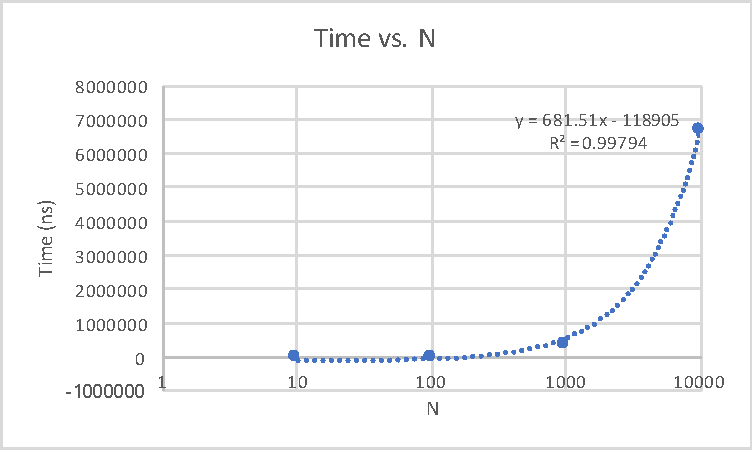
\includegraphics[scale=0.45]{ArrayMax.pdf}
        }{
          \caption{Time vs. N for ArrayMax}
        }
        \capbtabbox{
          \begin{tabular}{cc}
            \hline
            \textbf{N} & \textbf{Time (ns)} \\ \hline
            10         & 6000               \\
            100        & 27000              \\
            1000       & 346000             \\
            10000      & 6717000            \\ \hline
          \end{tabular}
        }{
          \caption{ArrayMax's data.}
        }
      \end{floatrow}
    \end{figure}

    \subsection{ArraySum}
    \begin{figure}[ht]
      \begin{floatrow}
        \ffigbox{
          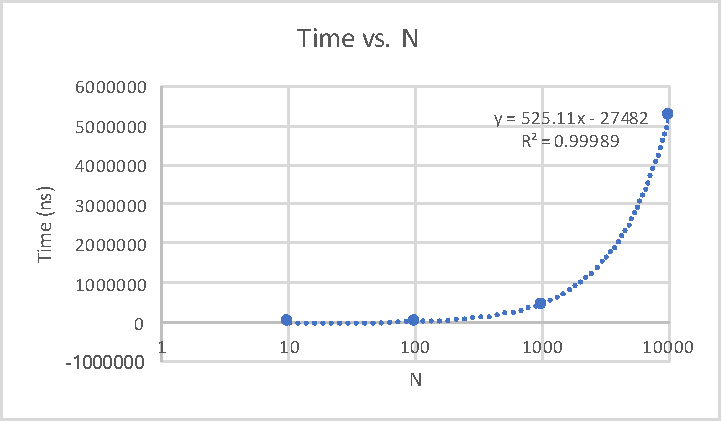
\includegraphics[scale=0.45]{ArraySum.pdf}
        }{
          \caption{Time vs. N for ArraySum}
        }
        \capbtabbox{
          \begin{tabular}{cc}
            \hline
            \textbf{N} & \textbf{Time (ns)} \\ \hline
            10         & 8000               \\
            100        & 26000              \\
            1000       & 463000             \\
            10000      & 5227000            \\ \hline
          \end{tabular}
        }{
          \caption{ArrayMax's data.}
        }
      \end{floatrow}
    \end{figure}

    \subsection{Fibonacci}
    \begin{figure}[ht]
      \begin{floatrow}
        \ffigbox{
          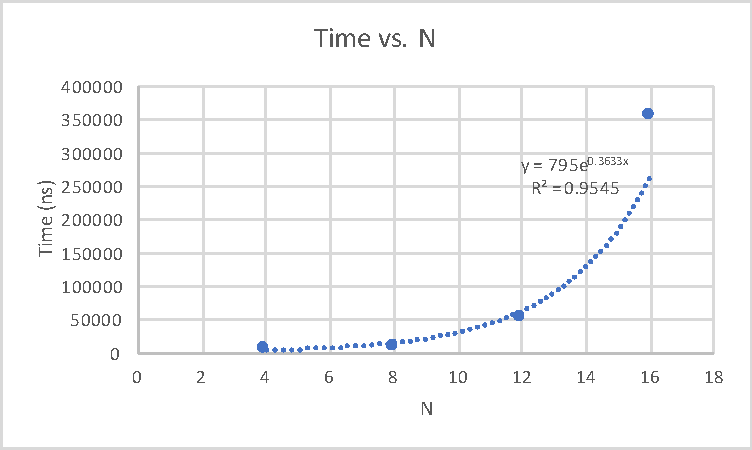
\includegraphics[scale=0.45]{Fibonacci.pdf}
        }{
          \caption{Time vs. N for Fibonacci}
        }
        \capbtabbox{
          \begin{tabular}{cc}
            \hline
            \textbf{N} & \textbf{Time (ns)} \\ \hline
            4         & 5000               \\
            8        & 9000              \\
            12       & 51000             \\
            16      & 356000            \\ \hline
          \end{tabular}
        }{
          \caption{ArrayMax's data.}
        }
      \end{floatrow}
    \end{figure}

    \subsection{What can you say between the experimental and theoretical results?}
    The graphs obtained by measuring time to resolve of each algorithm match at a good scale
    the theoretical values. The differences can be explained because the big $O$ notation only takes
    consideration to values that tend to infinity and, actually, although the used values are
    considerably big there are other terms that may affect the behaviour of the curve.
    \subsection{What did you learn about \texttt{Stack Overflow}?}
      The Stack Overflow error is caused by a bad recursive call -for example you do not make
      the problem simpler every time you make a recursive call- or when you do not have a stopping
      condition.\cite{StackOverflow} Java Stack memory is used for execution of a thread.
      Whenever a method is invoked, a new block is created in the stack memory for the method to hold
      local primitive values and reference to other objects in the method.\cite{HeapStack}
    \subsection{What's the biggest Fibonacci value you were able to compute? Why? Why are you not able to compute Fibonacci with 1 million?}
    The maximum Fibonacci number we could calculate was the 51th number of the series on our computers on
    a reasonable time; as a side note, we could calculate bigger values but the time of doing so isn't worth
    it compared to the computational cost. We couldn't calculate bigger for two reasons:
    \begin{enumerate}
    \item The time would be really big, as of lasting days or weeks to calculate.
    \item The ram of the computer has a limited space so, even if we set the stack size to a really big
    number, the memory consumed will eventually occupied the whole ram memory.
    \end{enumerate}
    The number of operations the computer has to do for big values is approximately in the order of
    an exponential base 2. In this manner, to calculate the millionth term of the series it would need
    around $2^{10^6}$, even if we had a 4 GHz computer processor the time it would take whould be
    $2^{10^6-2}*10^{-9}$. Additionally, if we had infinite time to calculate this term we cannot solve the
    problem that we do need finite memory to fill the stack memory for the recursion.

    \subsection{How can you compute Fibonacci of big values?}
    We can use Dynamic Programming. Dynamic Programming is a method to solve recursive algorithms more efficently;
    the main idea is to use \textbf{memoization}, where we have to store the solution of the subprocesses that the
    algorithm would have to repeat each time it is executed, in order not to solve them again. One approach to the
    solution using \textbf{memoization} is showed below: \cite{SJ}
    \begin{Verbatim}
    public int fibTopDown(int n) {
     if(n == 0) return 1;
     if(n == 1) return 1;
     if(fib[n] != 0) {
       return fib[n];
     } else {
      fib[n] = fibTopDown(n-1) + fibTopDown(n-2);
  	  return fib[n];
     }
    }
    \end{Verbatim}

    \subsection{What can you say between the complexity of \texttt{Recursion I} and \texttt{Recursion II} from \texttt{CodingBat}?}
    We can conclude that when we use one recursion, the complexity is n and, if we use two
    recursive calls, it is $2^n$. In general terms, we think it is safe to assume that
    for i recursion calls the complexity of the algorithm is $O(i^n)$.
    In \texttt{Recursion I} the complexity of all algorithms are $O(n)$; while in \texttt{Recursion II}
    the complexity of all the algorithms is $O(2^n)$

    \section{EXAM SIMULATION}
    \begin{enumerate}
      \item $\texttt{start}+1,\quad \texttt{nums},\quad \texttt{target}$
      \item a) $T(n) = T(n/2) + C$
      \item $n-a, a, b, c$\\
      res, solucionar($n-b,a,b,c$)+1\\
      res, solucionar($n-c,a,b,c$)+1
      \item e) La suma de los elementos de a y es $O(n)$.
    \end{enumerate}


    \newpage
    \bibliographystyle{plain}
    \bibliography{Lab.bib}
\end{document}
